\chapter*{Résumé détaillé en français}\setcounter{page}{1}

\textbf{Résumé.}%Context
La simplicité des chaînes de caractères et leur versatilité placent leur traitement au cœur de nombreuses applications, telles que la bio-informatique, la recherche d'informations et la cybersécurité.
Le problème naturel de la recherche exact de motifs a été largement étudié~\cite{charras2004handbook}, cependant, de nombreuses applications nécessitent également des requêtes plus complexes. Par ailleurs, dans les domaines applicatifs, la quantité d'informations à traiter augmente à une vitesse stupéfiante~\cite{muir2016real}, et les requêtes exactes ne sont pas toujours assez rapides.

%First part
Dans la première partie de cette thèse, nous étudions des requêtes complexes telles que la recherche par expressions régulières, la recherche de motifs consécutifs avec espacement et la détection de carrés.
%Regexp
Pour la recherche d'expressions régulières, nous donnons un algorithme efficace en espace dans le modèle de flot de données : les caractères du texte arrivent un par un, et nous ne pouvons accéder aux anciens que si nous les stockons explicitement.
%Gapped
Ensuite, la recherche de motifs consécutifs avec espacement est un type de requête plus simple où, étant donné deux motifs $P_1$, $P_2$ et un intervalle $[a, b]$, il faut signaler toutes les occurrences consécutives de $P_1$ suivies de $P_2$ espacés d'une distance dans $[a, b]$. Nous étudions ce problème dans plusieurs modèles : algorithme de flot, la recherche de motifs sur un texte compressé, et l'indexation compressée.
%Square
Nos solutions, pour les deux problèmes précédant, utilisent la détection périodicité pour s'épargner des calculs redondants. Cette utilisation de la périodicité rend les carrés intéressants à étudier au-delà de leur signification inhérente~\cite{Kolpakov2003}. Nous étudions la détection et le calcul des carrés pour alphabets généraux (le cadre le plus abstrait dans lequel les carrés peuvent être définis). Nous fournissons un algorithme optimal et répondons à une question ouverte posée en 1984 par Main et Lorentz~\cite{Main1984}.

% Second part
La seconde partie de cette thèse propose quelques utilisations d'approximations afin de passer à l'échelle sur des grandes quantités de données dans diverses applications, dont la bio-informatique.
%
Nous étudions tout d'abord la recherche approximative de motifs, où nous devons rapporter toutes les occurrences à une distance au plus égale à $k$ pour une mesure de similarité donnée.
% LCS DTW
%Motivés par les bornes inférieures pour le calcul des mesures de similarité les plus populaires,
Nous fournissons des algorithmes paramétrés efficaces pour calculer la longueur de la plus longue sous-chaîne commune avec environ $k$ différences, puis pour la recherche de motifs avec déformation temporelle dynamique. En raison de leur robustesse au bruit dans l'entrée, ces deux mesures peuvent être appliquées à la détection sections répétées dans un texte, nécessaire pour des applications telles que la détection de plagiat~\cite{zou2010cluster} et l'alignement de séquences biologiques~\cite{leimeister2014kmacs,loose2016real,han2018accurate}.
% XBWT
Enfin, nous proposons un index compressé pour des collections de lectures de séquençage redondantes, qui tire parti d'alignements sur un génome assemblé pour améliorer la compression, mais qui peut néanmoins donner lieu à des faux positifs dans les recherches.
\newpage

\section*{Contexte de la thèse}

Lorsque je réponds à la question classique ``Quel est le sujet de ta thèse ?'' posée par ma famille et à mes amis, je commence toujours par la fonction ``Ctrl + F'' dans leur éditeur de texte ou leur navigateur web préféré. Cela permet de mettre rapidement en évidence l'une des applications de la recherche exacte des motifs.
Mais même mes grands-parents savent immédiatement qu'une recherche efficace dans un texte est possible depuis des décennies et qu'il ne peut s'agir de mon véritable sujet de recherche.

En effet, le problème de la recherche exacte de motif dans un texte a été largement étudié, avec en particulier, le célèbre algorithme de Knuth--Morris--Pratt fait partie des algorithmes classiques. Charras et Lecroq ont publié un manuel détaillé~\cite{Charras2004} sur les différentes solutions pour la recherche exacte de motif dans un texte et ces solutions ont également été comparées dans le détail en pratique~\cite{DBLP:journals/corr/abs-1012-2547, faro2013exact}. En général, cependant, le besoin de traitement de texte va bien au-delà de la recherche exacte de motifs. Dans cette thèse, nous regroupons les problèmes de traitement de chaîne de caractères étudié en trois grandes catégories : la recherche de motifs complexes, le calcul de distance et mesure de similarité, et enfin la détection de répétitions. Nous détaillerons ensuite la nécessité d'avoir des algorithmes ultra-efficaces pour essayer de passer à l'échelle sur les grandes quantités de données des domaines applicatifs utilisant le traitement de chaînes de caractères.

\subsection*{Traitement des chaînes de caractères}

\noindent\textbf{Recherche de Motifs Complexes.}
% Regexp
L'un des modèles le plus utilisé et classique pour les requêtes complexes est \underline{la recherche par expressions régulières}, introduite par Kleene en 1951~\cite{RM-704}.
% Definition
Le formalisme des expressions régulières permet une description concise d'ensembles de chaînes par des combinaisons récursives de caractères d'un alphabet $\Sigma$ ainsi que de trois opérateurs fondamentaux : la concaténation ($\cdot$), l'union ($|$) et l'étoile de Kleene ($\ast$).
Pour deux expressions rationnelles $R_1$ et $R_2$, la concaténation $R_1\cdot R_2$ reconnaît toute concaténation d'une chaîne reconnue per $R_1$ et d'une chaîne reconnue par $R_2$, l'union $(R_1|R_2)$ reconnaît toute chaîne reconnue par $R_1$ ou $R_2$, et $(R_1)^\ast$ reconnaît toutes répétitions d'une chaîne reconnue par $R_1$, y compris l'absence de répétition, c'est-à-dire la chaîne vide.
% Applications
L'utilisation des expressions régulières a gagné en popularité dans les années 1970 grâce à leur mise en œuvre efficace dans les outils Unix tels que \texttt{awk}, \texttt{grep}, ou \texttt{sed}.
Elles sont devenues un outil crucial dans de nombreux domaines tels que l'analyse du trafic internet~\cite{4221791,4579527}, les bases de données, l'exploration de données~\cite{1000341,10.5555/645927.672035,10.1145/375551.375569}, les réseaux informatiques~\cite{10.1145/1159913.1159952}, et la recherche de protéines~\cite{10.1145/369133.369220}.
%
Nous étudions les expressions régulières dans le Chapitre~\ref*{chap:regexp}.

% Gapped matching
Malheureusement, Backurs et Indyk~\cite{DBLP:conf/focs/BackursI16} suivis par Bringmann, Gr{\o}nlund, et Larsen~\cite{8104068} ont prouvé des bornes inférieures conditionnelles qui impliquent que certaines expressions régulières ne peuvent probablement pas être recherchées en temps fortement sous linéaire.
% Ne se préoccupe pas
Comme alternative plus simple, Fischer et Paterson~\cite{FischerPaterson} ont introduit la recherche de motifs avec \underline{``don't care''} où un symbole don't care (aussi appelé wildcard ou gap), dénoté \texttt{?}, peut apparaître à la fois dans le motif et dans le texte, et correspond à n'importe quel autre caractère de l'alphabet.
% Graine d'espace
Ce modèle a été directement appliqué dans la base de données de protéines PROSITE~\cite{hulo2006prosite} où les caractères génériques sont pris en charge. Plus généralement, les space seeds~\cite{li2004patternhunter}, un concept similaire où seules certaines positions doivent corespondre, ont été utilisées dans la recherche d'homologie~\cite{ma2002patternhunter}, l'alignement~\cite{david2011shrimp2}, l'assemblage~\cite{birol2015spaced}, et la métagénomique~\cite{bvrinda2015spaced}.
% Correspondance par lacunes
Les motifs avec don't cares sont parfois~\cite{lewenstein2011indexing} décrits comme $P= P_1g_1P_2g_2 \dots g_\ell P_{\ell+1}$ où $P_1$,$P_2$, \dots,$P_{\ell+1}$ sont des motifs sur l'alphabet $\Sigma$ et $g_1,g_2,\dots,g_{\ell}$ sont le nombre de \texttt{?} entre deux motifs. 
% variable length gap
Naturellement, cette question a ensuite été étendue au problème de la recherche de motifs avec \underline{espacement variable}~\cite{bille2012string,bille2014string} où la longueur des espaces peut varier dans des intervalles $[a_i,b_i]$ pour $i\in[1,\ell]$.
% Applications
Les espacements de longueur variable sont également pris en charge par la base de données PROSITE~\cite{hulo2006prosite}.
% Variantes
Différentes variantes du problème ont été étudiées~\cite{kopelowitz2016color,cohen2009range,brodal1999finding}, y compris une version plus simple avec seulement deux motifs $P_1$ et $P_2$ et un seul espace~\cite{peterlongo2006gapped,iliopoulos2009indexing} et le cas spécial $P_1=P_2$~\cite{muthukrishnan2002efficient,keller2007range}.

% consécutif
En 2016, Navarro et Thankatchan~\cite{NAVARRO2016108} ont proposé une variante naturelle : étant donné un motif unique $P$ et un intervalle $[a,b]$, on doit déclarer toutes les occurrences \emph{consécutives} de $P$ commençant aux positions $(i,j)$ (consécutive signifiant aucune autre occurrence entre $i$ et $j$) tel que $j-i$ appartient à $[a,b]$. Depuis, les occurrences consécutives ont été étudiées dans plusieurs publications~\cite{DBLP:conf/fsttcs/BilleGPRS20,DBLP:journals/corr/abs-2304-00887,DBLP:journals/corr/abs-2211-16860}.
% Correspondance consécutive à espacement
Récemment, Bille et al.~\cite{bille2022gapped} ont proposés une combinaison des modèles de recherche de motifs consécutive et de recherche de motifs avec espacement : \underline{la recherche de motifs consécutifs avec espacement}.
% Definiton
Dans ce modèle que nous étudions dans les Chapitres~\ref*{chap:gapped_index} et~\ref*{chap:gapped_pm}, on nous donne deux motifs $P_1$, $P_2$ et un intervalle $[a, b]$, et il faut renvoyer toutes les occurrences consécutives (sans autres occurrences des motifs entre les deux) de $P_1$ suivies de $P_2$ espacés d'une distance dans $[a, b]$. 



\noindent\textbf{Mesures de Similarité.} 
% Mesures de similarité
De nombreuses applications de chaînes de caractères doivent composer avec la présence de bruit dans les données d'entrée, ce qui rend difficile la recherche de correspondances exactes. Les modèles tels que don't care et variable length gap matching présenté précédemment définissent leur match de manière à prendre en compte les données d'entrée bruitées, mais une autre approche consiste à travailler avec des distances et des mesures de similarité. La quantification du degré de similarité et de dissimilarité de deux chaînes de caractères est par exemple nécessaire en bio-informatique~\cite{Gusfield1997}, en analyse musicale~\cite{Mongeau1990} et en détection de plagiat~\cite{lukashenko2007computer}. 
%
Une mesure de distance quantifie la dissimilarité entre les chaînes de caractères, tandis qu'une mesure de similarité quantifie le degré de ressemblance entre les chaînes de caractères. La plupart des distances peuvent être dérivées en mesures de similarité, et la plupart des mesures de similarité ont une distance correspondante. Dans cette section, nous alternons donc les deux termes en fonction de la forme la plus courante dans la littérature.

% Robustesse au bruit
Différents types de bruit peuvent apparaître dans les données, tels que le remplacement, l'insertion ou la suppression de caractères, ou encore l'étirement ou la réorganisation de sections du texte. Par conséquent, diverses mesures de similarité peuvent être définies pour tenir compte des différents types de bruit, l'objectif étant toujours que quelques modifications ne changent pas radicalement la distance par rapport à d'autres chaînes de caractères.
% Hamming
L'une des distances les plus simples sur les chaînes de caractères est la distance de Hamming : Pour deux chaînes $X$ et $Y$ avec $|X|=|Y|$, il s'agit du nombre de différences entre $X$ et $Y$. La distance de Hamming est également définie comme le nombre de substitutions nécessaires pour transformer $X$ en $Y$.
% Longuest Common Subsequence (suite commune la plus longue)
Lorsque l'objectif est plutôt d'avoir une mesure de similarité robuste aux insertions et aux suppressions dans les chaînes $X$ et $Y$, on peut considérer la longueur de la \underline{plus longue sous-séquence commune} entre $X$ et $Y$ : le plus grand $\ell$ tel qu'il existe des positions $i_1<.... < i_\ell$ et $j_1< ... < j_\ell$ telles que $X[i_p] = Y[j_p]$ pour tout $p \in [1,\ell]$. Notez que la plus longue sous-séquence commune est à la base d'outils de comparaison tels que \texttt{diff} qui sont ensuite appliqués dans des systèmes de contrôle de version tels que git.
% ED / Levenshtein
Pour la distance de \underline{Levenshtein}~\cite{levenshtein1966binary} (également appelée distance d'édition par la suite), les opérations autorisées sont les substitutions, les insertions et les suppressions, toutes avec un coût de $1$. Cette définition peut être généralisée pour permettre aux coûts de différer pour chacune des opérations (distance d'édition pondérée) ou même pour que le coût dépende du caractère qui est ajouté, supprimé ou substitué (distance d'édition pondérée en fonction de l'alphabet). Cette métrique est l'une des plus connues, en raison de l'importance de la recherche d'alignements globaux (alignements de deux chaînes complètes avec substitutions, insertions et suppressions) en bio-informatique~\cite{Gusfield1997}.
Malheureusement, Backurs et Indyk~\cite{DBLP:conf/stoc/BackursI15} ont prouvé une borne inférieure conditionnelle (basée sur SETH) qui suggère qu'il est peu probable que la distance d'édition soit calculable en temps fortement sous-quadratique.
% LCS avec $k$ mismatchs
Pour tenter de contourner cette limite inférieure, dans le Chapitre~\ref{chap:LCS}, nous considérons la \underline{plus longue sous-chaîne  commune (LCS) avec environs $k$ différences} comme une version approximative d'une mesure résiliente aux substitutions : \underline{LCS avec $k$ différences}. Dans le problème LCS avec $k$ différences, étant donné un entier $k$ et deux chaînes $X$ et $Y$, $\lcsk(X,Y)$ est la longueur maximale d'une sous-chaîne (qui doit être continue, contrairement à une sous-séquence) de $X$ qui apparaît dans $Y$ avec au plus $k$ différences. 
Mais là encore, Kociumaka, Radoszewski et Starikovskaya~\cite{DBLP:journals/algorithmica/KociumakaRS19} ont montré (sous réserve de SETH) qu'il existe $k=\Theta(\log n)$ tel que LCS avec $k$ différences ne peut être résolu en temps fortement sous-quadratique, ils ont donc introduit LCS avec environs $k$ différences dans le but de rendre le problème plus facile par approximation.
Dans le Chapitre~\ref{chap:LCS}, nous étudions ce problème, où nous recevons une constante $\eps > 0$, et nous devons retourner une sous-chaîne de $X$ de longueur au moins $\lcsk(X,Y)$ qui apparaît dans $Y$ avec au plus $(1+\eps) \cdot k$ différences. Nous fournissons deux nouveaux algorithmes avec des compromis spatio-temporels différents et évaluons l'éficacité pratique de l'un d'entre eux par rapport à la solution de programmation dynamique quadratique pour LCS avec $k$ différences.


% Correspondance approximative
Outre la comparaison directe de deux chaînes de caractères, les distances sont également utilisées pour définir des problèmes de recherche approximative de motifs~\cite{landau1986efficient,landau1989fast} où, pour un entier donné $k$, un motif $P$ et un texte $T$, on doit trouver toutes les positions $j$ telles qu'il existe une sous-chaîne $T[i..j]$ qui est à une distance maximale de $k$ par rapport à $P$.
Pour un aperçu des résultats obtenus avant 2001 sur la recherche approximative pour les distances d'édition, de Hamming et de la plus longue séquence commune, voir~\cite{navarro2001guided}.
% DTW
Nous étudions l'appariement approximatif dans le Chapitre~\ref{chap:DTW} pour une distance populaire pour les séquences temporelles, qui est moins courante pour les chaînes de caractères : la \underline{Dynamic Time Warping (DTW) distance}~\cite{sakoe1978dynamic}. Pour les chaînes de caractères, la distance DTW peut être décrite comme suit : dupliquer certains caractères dans le but d'obtenir des chaînes de longueur égale et de minimiser la somme des distances entre les caractères situés aux mêmes positions, cette somme étant la distance DTW. Le calcul de la distance d'édition a été réduit au calcul de DTW~\cite{DBLP:conf/icalp/Kuszmaul19}.\\


\noindent\textbf{Détections de Répétitions.} Après avoir abordé les modèles de recherches de motifs et les mesures de similarité, nous passons maintenant à une autre tâche centrale du traitement des chaînes de caractères : la détection de répétitions. La localisation des fragments répétés dans une chaîne de caractères peut être utilisée pour détecter les données dupliquées qui doivent être supprimées ou pour compresser leur représentation. Par exemple, la décomposition d'une chaîne en fragments maximaux apparus précédemment est à la base de la factorisation de Lempel--Ziv~\cite{ziv1977universal}. Une fois détectées, les régions hautement répétitives d'une chaîne peuvent également être traitées différemment, permettant d'obtenir un algorithme plus efficace.

En musique~\cite{arom1989time}, génomique~\cite{pich2018somatic}, finance~\cite{harvey2007trends} et astronomie~\cite{hewish1979observation}\footnote{ Lorsque Jocelyn Bell a découvert pour la première fois des signaux provenant de pulsars (une étoile à neutrons en rotation qui crée un effet de phare), leurs régularités étaient si surprenantes que des spéculations ont été faites sur le fait qu'ils pourraient être des signaux d'une intelligence extraterrestre.}, de nombreuses données présentent des signes de répétitions et de phénomènes périodiques.
Formellement, on dit qu'une chaîne $T$ de longueur $n$ est périodique avec une période $p$ si pour tout $0 \leq i < n - p$, $T[i]=T[i+p]$, et la plus petite période de $T$ est simplement appelée la période de $T$.
%
Mais souvent, les données d'entrée ne contiennent que des sous-chaînes périodiques (au lieu d'être entièrement périodiques), ce qui conduit naturellement au concept de runs. Les runs sont des sous-chaînes maximales périodiques, c'est-à-dire qu'une sous-chaîne $T[i..j]$ est un run si elle est périodique avec une période $p$, et $T[i-1..j]$ et $T[i..j+1]$ (si elles sont bien définies, c'est-à-dire $0<i$ et $j<|T|-1$) ne sont pas périodiques avec une période $p$. 

Un modèle plus simple souvent considéré est le carré : des sous-chaînes $T[i..i+2k-1]$ telles que $T[i..i+k-1]=T[i+k..i+2k-1]$, on parle de carré ou de tandem. Cette forme de répétition est naturellement présente dans l'ADN et joue un rôle important dans l'établissement des empreintes génomiques~\cite{Kolpakov2003,GYMREK20179}. 
%
L'étude des carrés dans les chaînes de caractères remonte à 1906 avec les travaux de Thue~\cite{thue1906} sur la construction d'un mot infini sans carré. En termes d'algorithme, la question la plus fondamentale est de tester si une chaîne de longueur $n$ contient au moins un carré, et elle a été examinée pour la première fois par Main et Lorentz~\cite{Main1984} qui ont conçu un algorithme en temps $\Oh(n \log n)$. Ils ont utilisé une approche en ``diviser pour régner'' pouvant être adaptée pour obtenir une représentation compacte de tous les carrés dans le même temps. Ils ont également montré que $\Omega(n\log n)$ comparaisons (vérifier si deux caractères sont égaux) sont nécessaire pour tester la présence de carré sans ordre sur l'alphabet. Cependant, leur preuve utilise des chaînes avec jusqu'à $n$ caractères distincts et ils ont laissé explicitement ouverte la question de savoir si un algorithme plus rapide pouvait être conçu lorsque la taille de l'alphabet est restreinte. 
Dans le Chapitre~\ref{chap:squares}, nous montrons qu'en effet, pour une chaîne sur un alphabet non ordonné de taille $\sigma$, il existe un algorithme pour tester si elle contient un carré en temps $\Oh(n\log \sigma)$ n'utilisant que des tests d'égalité pour comparer les caractères. Nous montrons également que ce résultat est optimal pour les algorithmes déterministes et nous étendons notre solution pour permettre de renvoyer de toutes les runs de la chaîne.

\subsection*{Difficulté du Passage à l'Échelle}

% Mais il ne s'agit pas seulement du modèle spécifique, il s'agit aussi de l'extensibilité.
Nous avons vu jusqu'à présent comment les tâches de traitement des chaînes de caractères ont des applications cruciales pour d'autres domaines appliqués, mais un autre défi majeur dans la plupart des applications est le passage à l'échelle sur de grands jeux de données.
% Wikipedia
Les jeux de données manuellement gérés restent généralement de petite taille. Par exemple, les pages anglaises de Wikipédia (uniquement le texte et les métadonnées) occupaient 20~gigaoctets dans un format compressé en 2022~\cite{wikimedia}. En comparaison, toute forme d'archivage et d'historique des versions tend à être beaucoup plus volumineuse. Les métadonnées de l'historique des révisions (sans le contenu des articles) pour les pages anglaises de Wikipédia occupaient à elles seules 75~gigaoctets en 2022.
% Héritage logiciel
Il est parfois possible de limiter la redondance dans des données archivées, par exemple en utilisant un graphe indiquant les endroits où les données sont répétées. C'est l'approche adoptée par le projet Software Heritage~\cite{swh-site}, qui vise à archiver l'intégralité du code logiciel produit par l'humanité. La structure du graphe est particulièrement nécessaire dans ce projet pour refléter l'utilisation courante d'historiques de versions dans le développement de logiciels.
Des efforts considérables de recherche et d'ingénierie~\cite{DBLP:phd/hal/Pietri21} ont été déployés pour permettre une navigation efficace dans le graphe. 
Cependant, comme les dépôts de code sont indexés sur la base de leurs URL et de leurs métadonnées, il n'est actuellement pas possible d'effectuer une recherche spécifique pour trouver les occurrences d'un extrait de code particulier\footnote{\setlength\parindent{10pt} Un exemple simple mais intéressant est~\cite{vii2014if} où l'auteur a recherché \texttt{"const double epsilon ="} (et les équivalents dans d'autres langages) sur tous les dépôts GitHub pour étudier la valeur que les programmeurs choisissent généralement pour epsilon.}.
En 2023, le graphe est limité à 7~terabytes, mais avec les fichiers source, l'archive occupe proche de 1~petabyte~\cite{swh-polytechnique}.
% Archives Internet
Un autre exemple de grand projet d'archivage est l'Internet Archive, une organisation à but non-lucratif qui a commencé à sauvegarder des pages web en 1996 et qui détient aujourd'hui un historique pour plus de 800 milliards de pages web grâce à son programme : la Wayback Machine~\cite{web-archive}. Cette archive occupe plus de 70~pétaoctets et continue de grandir rapidement (voir Figure~\ref{fig:scalability_FR}).
Là encore, les options de recherche sont limitées aux métadonnées des sites web et non aux contenus des pages web elles-mêmes.

%%%%%%%%%% Bioinformatique
%Intro Représentation de l'ADN
De grandes archives de chaînes de caractères existent également en bio-informatique, mais la structure des séquences biologiques est très différente de celle de programmes ou de pages web, qui sont typiquement structurés, avec des liens, un grand alphabet et un nombre raisonnable de mots distincts.
% Introduction à l'ADN
L'information génétique codée dans l'ADN peut être abstraite comme une simple chaîne sur l'alphabet des nucléotides \texttt{\{A, T, C, G\}}.
Nous obtenons cette chaîne après séquençage et assemblage. Lorsqu'un génome est séquencé, le résultat est un ensemble de fragments, appelés \emph{lectures}, extraits de la séquence originale. Les lectures peuvent contenir des erreurs de séquençage, notamment des insertions, des suppressions et des substitutions de nucléotides. La longueur typique et le taux d'erreur des lectures varient en fonction des techniques de séquençage.
%
Dans tous les cas, la position originale de la lecture dans le génome est perdue pendant le séquençage et les lectures doivent être alignées et fusionnées afin de reconstruire le génome original, ce problème est appelé l'assemblage de séquences. Pour rendre cette reconstruction possible, les lectures sont extraites en quantités telles que chaque position du génome original est couverte plusieurs fois. Cela rend les ensembles de lectures plus grands et plus redondants que le génome assemblé. 
Une difficulté supplémentaire réside dans le fait que l'ADN est composé de deux chaînes de nucléotides complémentaires (appariement \texttt{A-T, C-G}). Au cours du séquençage, ces chaînes complémentaires sont détachées et traitées dans des directions opposées, et les lectures proviennent des deux. Ainsi, lors de l'assemblage ou de l'alignement sur une référence, il est nécessaire de prendre en compte le complément inversé d'une lecture.


% Redondance
Les applications bio-informatiques travaillent avec des séquences qui sont généralement redondantes, soit en raison de régions répétées au sein d'un génome (redondance intra-génome), soit en considérant plusieurs génomes (de la même espèce) qui partagent des parties de leurs génomes (redondance inter-génome).
% Index de séquences uniques 
L'exploitation de cette redondance est essentielle pour fournir des algorithmes efficaces, pour des problèmes tels que l'indexation d'une chaîne de caractères.
Si l'ADN est stocké sous la forme d'une chaîne de nucléotides \texttt{\{A, T, C, G\}}, il n'utilise que 2 bits par base, mais nécessite un parcours linéaire de l'ensemble de la chaîne pour rechercher un motif. 
L'arbre des suffixes est une structure classique qui permet une analyse plus efficace des séquences, mais qui nécessite 10 octets par base~\cite{navarro2016compact}, ce qui représente 30 gigaoctets pour un génome humain contenant 3,3 milliards de bases. 
Cela n'est pas envisageable pour les projets où des milliers de génomes ont été séquencés, comme le projet 1000 génomes~\cite{10002015global} achevé en 2015 et le projet 100K génomes~\cite{100Kgenomes} achevé en 2018. 
Heureusement, les structures de données compactes qui exploitent la redondance pour réduire l'utilisation de l'espace offrent un compromis intéressant : pour un génome humain, elles permettent de représenter la séquence et son arbre de suffixes en utilisant seulement 4 gigaoctets~\cite{navarro2016compact}.

% Moins cher = plus de séquençage
Les algorithmes efficaces sont essentiels pour la bio-informatique, car depuis 2008, on a assisté à une diminution drastique du coût du séquençage combiné à une augmentation du débit (plus rapide que prévu par la loi de Moore~\cite{muir2016real}), entraînant une augmentation massive des volumes d'ADN séquencés. 
% ENA
À ce jour, l'Archive européenne des nucléotides a accumulé plus de 50 pétaoctets~\cite{ena} de données de séquençage.
% SRA
Alors que le NCBI Sequence Read Archive possède plus de 73 pétabases~\cite{sra} de données, dont 38 pétabases en libre accès, et continue de croître, voir Figure~\ref{fig:scalability}. Cependant, comme pour le Software Heritage project et internet archive, dans l'ENA et le NCBI, les données sont indexées uniquement sur la base de leurs métadonnées.
% Lien vers cette thèse 
Dans le Chapitre~\ref{chap:XBWT}, nous proposons un index compact spécialement conçu pour les ensembles de lectures courtes, qui tire parti de l'entrée redondante pour obtenir une meilleure compression.

\begin{figure}
    \centering
    \begin{subfigure}[b]{0.45\textwidth}
        \begin{tikzpicture}
            \node (img) {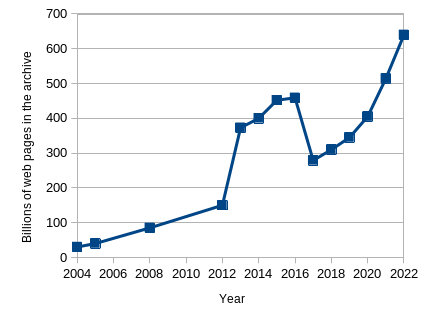
\includegraphics[width=0.95\textwidth]{0_sheets/wayback_machine.png}};
            \node [below right,text width=2.7cm,align=center, fill=white] at (0.25,-0.5){{\fontsize{7pt}{6pt}\selectfont Pages retirée pour des questions de sécurités.}};
            \draw[->] (1,-0.5) -- (1.3,0.3);
        \end{tikzpicture}
        \caption{The Wayback Machine Archive}
    \end{subfigure}
    \begin{subfigure}[b]{0.49\textwidth}
    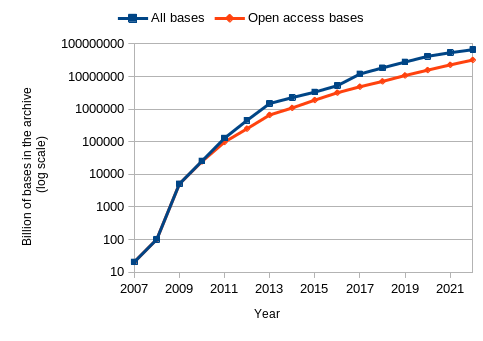
\includegraphics[width=\textwidth]{0_sheets/sra_growth.png}
    \caption{The Sequence Read Archive}
\end{subfigure}
\caption{
    Graphes de l'évolution des tailles de bases de données pour les archives the Wayback Machine~\cite{web-archive-growth} et the Sequence Read Archive~\cite{sra}. Ces bases donnés sont non seulement déjà très grandes, mais aussi grandissent toujours rapidement.
    }
\label{fig:scalability_FR}
\end{figure}

\section*{L'Utilisation de Sketches}

Jusqu'à présent, nous avons présenté les deux principaux défis au cœur du traitement de chaîne de caractère moderne : permettre des requêtes pertinentes (et parfois complexes) adaptées à des applications spécifiques tout en maintenant des performances qui permettent de passer à l'échelle sur de grands volumes de données.
%
Cette thèse propose de nouveaux compromis, théoriques et pratiques, entre les requêtes complexes et efficaces, et pour cela, nous nous reposons sur l'utilisation de \textbf{sketches}.
%
Dans cette thèse, un sketch est une compression avec ou sans perte qui ne conserve que les caractéristiques essentielles des données d'entrée nécessaires pour répondre à une requête donnée, offrant ainsi un potentiel prometteur pour le passage à l'échelle. 
% KR avec perte
Parmi les exemples de sketchs pour la compression avec perte, on peut citer les empreintes de Karp--Rabin~\cite{KRfingerprint} (voir Préliminaires~\ref{sec:prelim:KR}) qui occupent un espace constant et permettent de vérifier si deux chaînes de caractères sont égales avec une probabilité élevée, mais les empreintes ne contiennent pas en elles-mêmes suffisamment d'informations pour reconstruire les données d'origine.
% LZ sans perte
Pour la compression sans perte, un exemple est la factorisation de Lempel--Ziv~\cite{ziv1977universal}, une compression très efficace en pratique utilisée dans des formats de compression tels que \texttt{png} ou \texttt{zip}, qui permet toujours de reconstruire la chaîne de caractères originale, mais dans le pire des cas, la factorisation de Lempel--Ziv peut occuper autant d'espace que l'entrée d'origine.

\section*{Contributions}

La \textbf{Partie ~\ref{part:complex_queries}} se concentre sur une étude théorique des requêtes complexes.
% Expressions régulières
Nous commençons par la recherche d'expressions régulières dans le modèle des données en streaming.
%
Nous supposons que l'on nous donne une expression régulière $R$, un texte en streaming $T$ de longueur $n$. Pour le problème d'\emph{appartenance} à une expression rationnelle, nous devons déterminer, après avoir vu $T$ entièrement, s'il est reconnu par l'expression rationnelle $R$, tandis que pour \emph{recherche}, nous devons répondre, à chaque position $r$, s'il existe une sous-chaîne $T[l..r]$ reconnue par $R$.
% Parler des bornes inférieures ?
% Contribution principale
Dans le \textbf{Chapitre~\ref{chap:regexp}}, notre principale contribution est d'identifier $d$, le nombre de symboles d'union et d'étoiles de Kleene dans $R$, comme le paramètre clé qui permet un algorithme de streaming efficace en espace. 
% Utilisations antérieures du paramètre
Auparavant, Bille et Thorup~\cite{doi:10.1137/1.9781611973075.104}\footnote{Ils considèrent en fait $k$, le nombre de chaînes de caractères apparaissant dans $R$, mais $k=\Theta(d)$. } avaient déjà utilisé ce paramètre pour proposer des algorithmes permettant de résoudre l'appartenance et la recherche d'une expression régulière de longueur $m$ en $\Oh(m)$ espace et $\Oh(n(\frac{d\log w}{w} + \log d))$ temps, où $w$ est la taille du mot machine. Mais il restait à savoir si $d$ pouvait être utilisé pour une solution efficace en termes d'espace.
%
Nous répondons à cette interrogation en fournissant des algorithmes randomisés Monte Carlo (le temps d'exécution est déterministe, mais les algorithmes peuvent se tromper avec une faible probabilité) permettant de résoudre les problèmes d'appartenance et de recherche d'une expression régulière en espace $\Oh(d^3\polylog n)$ et un temps par caractère en $\Oh(nd^5\polylog n)$ (Théorème~\ref{th:memb}).

Voici un bref résumé de la façon dont nous prouvons notre résultat : nous commençons par définir \emph{chaînes atomiques} qui sont les ``mots'' apparaissant dans l'expression régulière. Elles ne contiennent que des caractères de $\Sigma$ et il y en a $\Theta(d)$. Par exemple, pour $R= \mathrm{GAT}(\mathrm{TA} | \mathrm{O})(\mathrm{CAT})^*$ l'ensemble des chaînes atomiques est $\{$GAT, TA, O, CAT$\}$.
%
La base de notre approche consiste à stocker efficacement certaines occurrences des préfixes des chaînes atomiques dans le texte $T$. Ces occurrences stockées sont ensuite liées pour tester s'il existe une correspondance ``partielle'' de $R$ (Définition~\ref*{def:partial_occ_regexp}).
Sur les régions périodiques du texte, il peut y avoir trop d'occurrences pour toutes les stocker.
Nous choisissons donc de ne stocker que quelques-unes de ces occurrences qui peuvent être très éloignées les unes des autres, avec juste une longue sous-chaîne périodique entre les deux. Pour reconstruire une correspondance partielle, nous devons vérifier si cette longue sous-chaîne périodique correspond à une exécution de l'automate de Thompson~\cite{Thompson_automaton}. Nous formulons cela comme la recherche d'un chemin de poids spécifique dans un multigraphe. Nous résolvons ensuite efficacement ce problème de graphe en le traduisant en un circuit utilisant des portes d'addition et de convolution qui peuvent être évaluées de manière efficace en termes d'espace à l'aide d'un système général~\cite{LokshtanovN10,Bringmann17}. En outre, nous améliorons ce système en supprimant sa dépendance à l'Hypothèse de Riemann étendue (Théorème~\ref{thm:bombieri}). 
%
Les sketches utilisés dans ce chapitre sont des empreintes de Karp--Rabin (Preliminaries~\ref{sec:prelim:KR}) utilisées pour détecter les occurrences des préfixes des chaînes atomiques, elles sont cachées dans l'algorithme de recherche de motifs (Théorème~\ref{th:pattern_matching}) que nous utilisons.\\

Dans le \textbf{Chapitre~\ref{chap:gapped_index}}, nous commençons notre étude de la recherche de motifs consécutifs avec espacement. Dans ce problème, on nous donne deux motifs $P_1$, $P_2$, et un intervalle $[a,b]$ et nous devons trouver toutes les paires de positions $(i,j)$ dans un texte $T$ telles qu'une occurrence de $P_1$ commence à la position $i$, une occurrence de $P_2$ commence à la position $j$, il n'y a pas d'occurrence de $P_1$ ou $P_2$ commençant dans l'intervalle $[i+1,j-1]$, et enfin $j-i \in [a,b]$.
%
Bille et al.~\cite{bille2022gapped} ont introduit ces requêtes et ont donné une borne inférieure conditionnelle indiquant que pour les index (texte traité en amont et les motifs donné ensuite sous forme de requêtes) de taille $\tilde \Oh(|T|)$ (la notation $\tilde \Oh$ cache les facteurs polylogarithmiques), l'obtention d'un temps de requête plus rapide que $\tilde \Oh(|P_1|+|P_2|+\sqrt{|T|})$ contredirait the Set Disjointness conjecture, même si $a=0$ est fixé. En outre, ils ont fourni une borne supérieure non-triviale qui utilise $\tilde \Oh(|T|)$ d'espace et $\tilde \Oh (|P_1| +|P_2| + |T|^{2/3}\occ^{1/3})$ de temps pour rapporter toutes les $\occ$ occurrences.

Nous supposons $a=0$ fixé, et que le texte $T$ de taille $n$ est donné comme un programme linéaire $G$ de taille $g$. Un programme linéaire est une grammaire sans contexte générant exactement une chaîne de caractères. Par exemple, la grammaire avec les non-terminaux $\{A,B,C,D\}$ et les règles $\{A \rightarrow BC, B \rightarrow b, C \rightarrow DD, D\rightarrow d \}$ génère la chaîne de caractères \texttt{bdd}.
Nous avons choisi ce formalisme, car il permet de capturer la populaire factorisation de Lempel--Ziv à un facteur logarithmique près : une factorisation de Lempel--Ziv de taille $z$ peut être transformée en un programme linéaire de taille $\Oh(z\log n)$~\cite{CharikarLLPPRSS02,Rytter02}.
%
Notre contribution est de créer un index prenant un espace polynomial dans la taille de la grammaire qui rapporte les occurrences consécutives à distance dans $[0,b]$ en temps optimal, à des facteurs polylogarithmiques près.
Pour rapporter les occurrences consécutives (sans contraintes sur la distance entre $P_1$ et $P_2$), notre index utilise un espace en $\Oh(g^2\log^4|T|)$ où $g$ est la taille de la grammaire (voir Corollaire~\ref{cor:all}).
%
Nous nous appuyons sur une construction efficace d'arbre à préfixes compactes (voir Preliminaries~\ref{sec:prelim:tries}) qui tire parti du fait que les chaînes sont des préfixes et des suffixes de chaînes générées par des non-terminaux. Cette implémentation utilise les empreintes de Karp--Rabin (voir Préliminaires~\ref{sec:prelim:KR}) et les arbres préfixes compactés sont ensuite augmentés à l'aide d'une décomposition en chemins de poids lourds.
Nous réutilisons ensuite cette structure pour notre résultat principal : Théorème~\ref{thm:close_co_occurrences}, avec un index qui rapporte des occurrences consécutives à distance dans un intervalle $[0,b]$ en utilisant l'espace $\Oh (g^5\log^5(|T|))$.
%
Le programme linéaire donné en entrée est le principal sketch utilisé dans ce travail, mais l'index que nous construisons forme également un sketch de la grammaire spécifique à la recherche d'occurrences consécutives.
%
L'index du Théorème~\ref{thm:close_co_occurrences} contourne la borne inférieure dans le cas des textes hautement compressibles (tels que $g^5 << n^2$). Il s'agit d'un résultat non-trivial puisque certains problèmes ne peuvent échapper à une forte dépendance vis-à-vis de la taille de la chaîne non compressée. Cependant, nous nous attendons à ce que notre complexité en espace soit loin d'être optimale et nous laissons les améliorations ainsi que le cas général avec $0 \leq a \leq b \leq |T|$ comme des questions ouvertes.


Partiellement motivés par les contraintes d'espace de notre index en $\tilde \Oh(g^5)$, dans le \textbf{Chapitre~\ref{chap:gapped_pm}}, nous abordons le problème dual : la recherche de motifs consécutifs. Dans ce problème, les motifs et le texte arrivent et sont traités en même temps. Notons que pour un texte non compressé, la recherche de motifs consécutifs peut être résolue par un algorithme de recherche linéaire classique, en gardant simplement la trace des occurrences les plus récentes de $P_1$ et $P_2$ en temps $\Oh(|T|+|P_1|+|P_2|+\occ)$ .
% Résultats
Nous montrons qu'une complexité similaire peut être atteinte lorsque le texte est hautement compressible : toutes les occurrences consécutives peuvent être rapportées en temps $\Oh(g+|P_1|+|P_2|+\occ)$ (voir le Théorème~\ref{th:main}) où $g$ est la taille du texte compressé sous forme de grammaire. Nous dérivons ensuite de ce résultat des algorithmes pour la recherche d'occurrences consécutives avec espacement (Corollaire~\ref{cor:ab}) et pour la recherche des k occurrences consécutives les plus proches (Corollaire~\ref{cor:topk}).
%
Notre résultat est basé sur l'encodage efficace de l'``information frontalière'' récemment introduit par Ganardi et Gawrychowski~\cite{DBLP:conf/soda/GanardiG22}. Pour un motif donné $P$, les informations $P$-frontalières d'une chaîne $S$ stockent les sous-chaînes apparaissant à la fois dans $P$ et $S$. Elles sont choisies pour capturer uniquement les informations nécessaires à la détection de nouvelles occurrences de $P$ qui pourraient survenir lors de la concaténation d'une chaîne à $S$. 
%
Les auteurs montrent comment utiliser cet encodage pour déterminer en $\Oh(g+|P|)$ temps si $P$ apparaît dans le texte compressé. Nous étendons leur approche pour rapporter toutes les occurrences croisant la frontière (Lemme~\ref{lemma:crossing}). Nous répétons ensuite cette technique à un deuxième niveau avec des ``informations frontalières secondaires'' et analysons soigneusement tous les cas pour obtenir le Théorème~\ref{th:main}. Ici encore, le sketch principal est la grammaire sur laquelle nous travaillons.\\


% Squares
Tous les chapitres précédents s'appuient fortement sur la détection de la périodicité pour le design des algorithmes, et il semblait donc naturel d'étudier ce problème dans le \textbf{Chapitre~\ref{chap:squares}}. Nous montrons comment rapporter tous les carrés en temps optimal dans le modèle le plus abstrait où ils peuvent être définis : les alphabets généraux (non ordonnés) où la seule opération autorisée est un test d'égalité entre deux caractères. 
Nous considérons d'abord le problème de la détection des carrés, puis nous étendons notre approche pour rapporter les carrés et runs.
% 
En 1984, Main et Lorentz~\cite{Main1984} ont conçu un algorithme en $\Oh(n\log n)$ temps pour la détection de carrés dans un texte $T$ de taille $n$ sur un alphabet général non ordonné. Ils ont également fourni une borne inférieure correspondante pour les chaînes ayant $\Omega(n)$ symboles distincts, mais ont laissé ouverte la question de savoir si un algorithme plus rapide était possible si la taille de l'alphabet $\sigma=|\Sigma|$ était restreinte.
% 
Nous commençons par prouver que le problème nécessite $\Omega(n \log \sigma)$ comparaisons même si la taille de l'alphabet est connue (Théorème~\ref{thm:lowerbound}). En outre, dans le Théorème~\ref{thm:inapproxalph}, nous montrons que le calcul de toute approximation pertinente du nombre de caractères distincts nécessite $\Omega(n\sigma)$ opérations.
%
Pour les alphabets ordonnés généraux (lorsqu'un ordre est donné), Crochemore~\cite{Crochemore1986} a utilisé la factorisation $f$ (liée à la factorisation de Lempel--Ziv) pour donner un algorithme de détection des carrés fonctionnant en temps $\Oh(n\log \sigma)$. En très résumé, la factorisation $f$ et la factorisation Lempel--Ziv (factorisation LZ) détectent les fragments répétitifs dans le texte et peuvent être calculées efficacement à l'aide d'un arbre à suffixes ou d'un tableau à suffixes. Cependant, nous montrons que pour les alphabets généraux non ordonnés, ces factorisations nécessitent $\Omega(n\sigma)$ opérations pour être calculées (corollaire de la borne inférieure sur l'approximation de l'alphabet). 
% 
Au lieu de cela, nous introduisons la factorisation de Lempel--Ziv $\Delta$-approchée qui agit comme un sketch capturant uniquement les carrés suffisamment longs (d'une longueur d'au moins $8\Delta$), par opposition à la factorisation $f$ et à la factorisation LZ qui capturent tous les carrés.
Nous présentons notre algorithme final par étapes. Nous supposons d'abord que la taille de l'alphabet est connue et nous nous concentrons sur l'obtention d'une borne supérieure sur le nombre de comparaisons, puis nous supprimons l'hypothèse de la connaissance de la taille de l'alphabet, et enfin nous fournissons un algorithme global efficace fonctionnant en temps $\Oh(n \log \sigma)$.\\


% Partie 2
La \textbf{Partie~\ref{part:approx-bio}} explore l'utilisation d'approximations pour réduire encore la taille des sketches et fournir des algorithmes encore plus efficaces. Chaque Chapitre fournit une implémentation pratique de ses algorithmes pour des applications en bio-informatique.
%
Plus tôt, nous avons détaillé l'importance des mesures de similarité pour de nombreuses applications.
%
En bio-informatique, la distance d'édition est sans doute la mesure de similarité la plus populaire, mais Backurs et Indyk~\cite{DBLP:conf/stoc/BackursI15} ont prouvé une borne inférieure conditionnelle (basée sur SETH) suggérant qu'il est peu probable que la distance d'édition soit calculable en temps fortement sous-quadratique.
%
La nécessité de surmonter cet obstacle a conduit à l'étude d'algorithmes approximatifs pour la distance d'édition. Chakraborty et al.~\cite{DBLP:conf/focs/ChakrabortyDGKS18} ont donné le premier résultat avec un algorithme d'approximation à facteur constant qui calcule la distance d'édition entre deux chaînes de longueur $n$ en temps $\tilde{\Oh}(n^{2-2/7})$.
Depuis notre publication~\cite{DBLP:conf/cpm/GourdelKRS20} (présentée dans le Chapitre~\ref{chap:LCS}), une série de travaux ont été publiés sur l'approximation de la distance d'édition~\cite{brakensiek2020constant,koucky2020constant}, le résultat le plus fort étant~\cite{andoni2020edit} avec une approximation à facteur constant en temps $n^{1+\eps}$ pour tout $\eps>0$ (où la constante d'approximation dépend uniquement de $\eps$).
Néanmoins, ces algorithmes ont tendance à être assez techniques et même ceux qui sont censés être plus simples, comme~\cite{andoni2020simple}, ne semblent pas avoir été implémentés et évalués dans la pratique.
%
Dans le \textbf{Chapitre~\ref{chap:LCS}}, nous adoptons une autre approche en considérant une mesure de similarité différente censée être à la fois robuste aux changements légers et suffisamment simple pour permettre un calcul efficace. Nous considérons la plus longue sous-chaîne commune (abrégée LCS par la suite) avec environ $k$ différences, qui est une version approximative de \kLCS. Rappelons que, pour un entier $k$ et deux chaînes $X$ et $Y$, $\lcsk(X,Y)$ est la longueur maximale d'une sous-chaîne de $X$ qui apparaît dans $Y$ avec au plus $k$ différences.
Pour une constante $\eps > 0$, le problème LCS avec environ $k$ différences doit retourner une sous-chaîne de $X$ de longueur au moins $\lcsk(X,Y)$ qui apparaît dans $Y$ avec au plus $(1+\eps) \cdot k$ différences. Ce problème a été introduit par Kociumaka, Radoszewski et Starikovskaya~\cite{DBLP:journals/algorithmica/KociumakaRS19} après qu'ils aient montré qu'il existe $k=\Theta(\log n)$ tel que \kLCS ne peut pas être résolu exactement en temps fortement sous-quadratique (conditionné par SETH).
% Notre contribution
Dans le Théorème~\ref{th:klcs_upper}, nous fournissons deux algorithmes : l'un supposant un alphabet de taille constante s'exécutant en $\Oh(n^{1+ 1/(1+2\eps) + o(1)})$ temps et en espace, et l'autre en $\Oh(n^{1+1/(1+\eps)} \log^3 n)$ temps et en espace linéaire sans contraintes sur l'alphabet. Le premier résultat repose sur une structure de données pour la recherche de plus proches voisins~\cite{DBLP:conf/stoc/AndoniR15} comme boîte noire, et nous ne l'évaluons pas dans la pratique. En revanche, notre deuxième contribution est plus simple et nous confirmons son caractère pratique par une évaluation expérimentale.
En outre, dans le Fait~\ref{lm:klcs_lower}, nous montrons une borne inférieure conditionnelle pour LCS avec environ $k$ différences (avec une construction similaire à la preuve de la borne inférieure de \kLCS ).
% Sketches
Dans nos algorithmes, nous nous appuyons sur les empreintes de Karp--Rabin et sur un sketch estimant la distance de Hamming basée sur la réduction de dimensions, tous deux détaillés dans la section~\ref{lcs:sec:prelim}. \\


% DTW
En poursuivant notre exploration des mesures de similarité et des distances, le Chapitre suivant se concentre sur la distance DTW (Dynamic Time Warping). Pour la distance DTW, il faut ``doubler'' les deux chaînes de caractère jusqu'à ce que les chaînes soient de même longueur, puis additionner les distances entre les caractères situés aux mêmes positions.
% RLE / Esquisses
Pour proposer un algorithme efficace pour cette distance, dans le \textbf{Chapitre~\ref{chap:DTW}}, nous considérons l'une des formes les plus simples de sketchs : l'encodage par plages (run-length encoding). L'encodage par plages d'une chaîne $S$ de longueur $N$ est défini comme $\RLE(S)=(c_1,l_1)(c_2,l_2)... (c_n,l_n)$ où $(c_i,l_i)$ représente le caractère $c_i \in \Sigma$ répété $l_i$ fois pour $i \in [1,n]$, et tel que $\sum_{i\in [1,n]} l_i = |S|$.
Ce sketch est particulièrement pertinent pour la DTW car les séries de caractères égaux ont tendance à être alignées malgré les variations de longueur. C'est pourquoi Froese et al.~\cite{DBLP:journals/corr/abs-1903-03003} ont déjà utilisé le nombre de runs dans les chaînes de caractères pour donner un algorithme calculant la distance DTW entre deux chaînes de caractères avec un temps d'exécution $\Oh(mN+nM)$, où $M,N$ sont la longueur des chaînes de caractères, et $m, n$ sont les tailles de leurs encodages par plage.

% Notre contribution 
Notre contribution est la suivante : lorsque les distances entre les caractères de $\Sigma$ sont des entiers, pour un motif $P$ avec $m$ runs et un texte $T$ avec $n$ runs, nous montrons qu'il existe un algorithme en $\Oh(n+m)$ temps qui calcule toutes les positions $j$ où la distance DTW entre $P$ et un suffixe de $T[..j]$ est au plus de 1. Puis, plus généralement, pour un entier $k$, nous fournissons un algorithme en temps $\Oh(knm)$ qui calcule toutes les positions $j$ où la distance DTW entre $P$ et un suffixe de $T[..j]$ est au maximum de $k$.
% Motivation bio
Notre intérêt et nos recherches sur DTW sont également motivés par des applications potentielles à l'analyse de données biologiques produites par le séquençage de troisième génération. Pour cette technologie, l'ADN passe à travers un nanopore à une vitesse irrégulière, ce qui tend à créer des erreurs dans la longueur des plages du même nucléotide (homopolymères)~\cite{delahaye2021sequencing}. Nous détaillons cette application potentielle dans la section~\ref{dtw:sec:experiments}.
% Mise à jour
Depuis notre publication, Boneh, Golan, Mozes, et Weimann ont mis en ligne une prépublication~\cite{boneh2023near} avec un temps en $\tilde{\Oh}(n^2)$ pour le calcul de la distance DTW entre deux chaînes avec $n$ runs, ce qui est optimale à des facteurs logarithmiques près. Ils suivent l'approche que Clifford et al.~\cite{clifford2019rle} ont utilisée pour montrer un résultat similaire pour la distance d'édition : ils représentent et traitent les entrées et les sorties à l'aide d'une fonction linéaire par morceaux.\\

% XBWT
Pour le \textbf{Chapitre~\ref{chap:XBWT}}, nous quittons l'étude des mesures de similarité pour nous concentrer sur le problème pratique de l'indexation des ensembles de lectures de séquençage. 
% Approximation
De plus, dans ce Chapitre, la perspective sur l'approximation est différente. Au lieu d'étudier la correspondance approximative où l'on rapporte toutes les sous-chaînes à une distance donnée du motif, nous proposons un index compact qui a l'inconvénient de rapporter des faux positifs : des occurrences du motif qui ne sont pas entièrement incluses dans une lecture.
%
Une lecture est une séquence de paires de bases, généralement courte (la longueur précise dépend de la technique de séquençage), obtenue lors du séquençage de l'ADN. Pour pouvoir réassembler l'ensemble de la séquence d'ADN, chaque position de la séquence est généralement couverte par plusieurs lectures. Le nombre moyen de lectures couvrant une position est appelé couverture de séquençage.
La couverture de séquençage standard pour les lectures courtes dans le but d'assembler un génome se situe aujourd'hui entre 30 et 50, ce qui rend les ensembles de lectures très répétitifs, en particulier lorsque l'ADN séquencé provient d'un seul individu.
%
Pour indexer une chaîne répétitive unique, l'index FM~\cite{ferragina2005indexing} basé sur la transformation de Burrows-Wheeler (BWT)~\cite{burrows1994block} est l'une des structures de données les plus importantes, et elle a été appliquée dans plusieurs outils bio-informatiques pour l'alignement des lectures courtes~\cite{langmead2009ultrafast,langmead2012fast,li2009fast}.
%
L'amélioration la plus récente du FM-index est le $r$-index de Gagie et al.~\cite{gagie2020fully} qui occupe un espace proportionnel à $r$, le nombre de plages dans la BWT de la chaîne indexée. Plus précisément, la structure de données occupe $\Oh(r\log\log n)$ d'espace tout en étant capable de compter et de localiser toutes les occurrences d'un motif en un temps optimal ( à un facteur logarithmique près). Cela fait du nombre de plages dans la BWT un paramètre important pour les structures économes en espace et $r$ est souvent considéré comme une mesure de la répétitivité du texte.
%
Malheureusement, l'extension de la BWT à une collection de chaînes de caractères n'est pas simple. Nous recommandons au lecteur la publication de Cenzato et Lipták~\cite{cenzato_et_al_BWT_Collections} qui présente toutes les variantes existantes pour construire une structure de type BWT pour une collection de chaînes et l'impact sur le nombre de plages dans la transformation qui en résulte.

Notre travail dans le Chapitre~\ref{chap:XBWT} propose de tirer parti d'une information très couramment associée aux lectures : l'alignement sur un génome de référence. Nous construisons un arbre dont le tronc principal est la référence et les lectures se ramifient à partir du tronc depuis la position sur laquelle elles sont alignées, puis nous calculons la généralisation de la BWT pour les arbres : la transformée de Burrows--Wheeler étendue (XBWT)~\cite{ferragina2009compressing}. Intuitivement, notre transformation fournit un contexte aux lectures qui permet un meilleur tri et limite le nombre de ruptures dans les plages de la chaîne transformée. Formellement, nous montrons que si les lectures sont presque identiques à la référence et que les différences sont situées vers la fin des lectures (ce qui est le cas en pratique pour les lectures courtes), le nombre de plages dans la XBWT peut être limité en fonction du nombre de plages dans la BWT de la référence. Nous testons ensuite notre approche en pratique et montrons qu'elle permet d'obtenir moins de résultats que la BWT avec l'heuristique co-lexicographique populaire (15\% de moins pour un ensemble de lectures du chromosome 19 humain).
% Fausses Positions
Le principal inconvénient de notre index est que nous cherchons dans l'arbre de branchement et donc, lorsque nous comptons le nombre d'occurrences d'un motif, nous ne pouvons pas éviter de compter les occurrences qui ne sont pas entièrement contenues dans une lecture (qui sont partiellement ou entièrement dans le tronc principal correspondant à la référence).
%
Une autre contribution de notre travail est que, dans le but de permettre un passage à l'échelle de la construction de l'index, nous adaptons la technique de découpage sans préfixe pour la construction de la BWT inventé par Boucher et al.~\cite{boucher2019prefix} à la construction de la XBWT. 
%
Dans la construction de la BWT par découpage sans préfixe, la chaîne d'entrée est découpée en phrases qui se chevauchent comme suit : nous maintenons un hash d'une fenêtre coulissante en utilisant les empreintes de Karp--Rabin, et chaque fois que le hash est égal à zéro, nous terminons la phrase en cours et en commençons une nouvelle. Cette technique, nous permet de créer un ensemble de phrases sans préfixe.
La chaîne est ensuite décomposée en un \emph{dictionnaire} et d'un \emph{parse}. 
Le dictionnaire associe chaque phrase à un métacaractère, et le parse est une chaîne de métacaractères.
Cette construction utilise des sketches (empreintes digitales de Karp--Rabin) mais crée également un sketch par le biais de cette représentation compacte de la chaîne.
L'intuition est que les sections répétées de la chaîne se traduiront par des phrases répétées qui peuvent être représentées par les mêmes métacaractères dans le parse, ce qui permet au dictionnaire de rester raisonnablement petit.
La BWT de la chaîne d'entrée est alors construite à partir de la BWT du parse (où l'ordre entre les métacaractères est l'ordre lexicographique de la phrase qu'ils représentent) et de la BWT des phrases.

L'adaptation de cette technique aux arbres et à la construction de la XBWT n'est pas triviale car chaque branche peut créer de nouvelles phrases. Nous avons implémenté notre index et l'avons évaluée expérimentalement en termes de nombre d'exécutions dans la XBWT résultante. La mise en œuvre des requêtes et l'analyse des faux positifs font partie des travaux futurs.

J'espère que cet aperçu des contributions a clairement mis en évidence le fait que les sketches sont des outils précieux dans de nombreux contextes et applications. Je m'attends à ce qu'ils continuent se développer dans de nombreux travaux futurs, tant en théorie qu'en pratique.